% fig_ejer1c_sum.tex — Componentes de x3(t) = 2u(t) - tu(t) + (t-2)u(t-2)
\documentclass[tikz]{standalone}
\usepackage{pgfplots}
\usepgfplotslibrary{groupplots}
\pgfplotsset{compat=1.18}
\definecolor{utnblue}{RGB}{0,102,204}
\definecolor{utnred}{RGB}{204,0,0}
\definecolor{utngreen}{RGB}{0,153,76}

\begin{document}
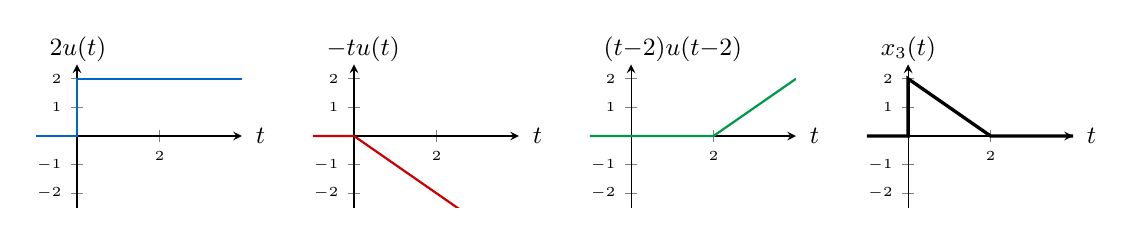
\begin{tikzpicture}
    \begin{groupplot}[
        group style={group size=4 by 1, horizontal sep=0.9cm},
        width=4.2cm, height=3.4cm,
        axis lines=middle,
        xmin=-1, xmax=4, ymin=-2.5, ymax=2.5,
        xtick={0,2}, ytick={-2,-1,0,1,2},
        xticklabel style={font=\tiny}, yticklabel style={font=\tiny},
        every axis plot/.append style={thick},
        every axis x label/.append style={at={(ticklabel* cs:1.02)}, anchor=west, font=\small},
        every axis y label/.append style={at={(rel axis cs:0.02,0.95)}, anchor=south west, font=\small},
    ]
    % Componente 1: 2u(t)
    \nextgroupplot[ylabel={$2u(t)$}, xlabel={$t$}]
    \addplot[utnblue] coordinates {(-1,0)(0,0)(0,2)(4,2)};

    % Componente 2: -tu(t)
    \nextgroupplot[ylabel={$-tu(t)$}, xlabel={$t$}]
    \addplot[utnred] coordinates {(-1,0)(0,0)(4,-4)};

    % Componente 3: (t-2)u(t-2)
    \nextgroupplot[ylabel={$(t{-}2)u(t{-}2)$}, xlabel={$t$}]
    \addplot[utngreen] coordinates {(-1,0)(2,0)(4,2)};

    % Suma total
    \nextgroupplot[ylabel={$x_3(t)$}, xlabel={$t$}]
    \addplot[black, very thick] coordinates {(-1,0)(0,0)(0,2)(2,0)(4,0)};
    \end{groupplot}
\end{tikzpicture}
\end{document}
